\section{Theorie}
\label{sec:Theorie}
Der Zustand oder die Phase eines Stoffes wird durch seine Temperatur und den auf diesen wirkenden Druck charakterisiert werden.
Damit hat der Stoff zunächst zwei Freiheitsgrade, mit denen dieser sich im Phasendiagramm \ref{fig:phasendiagramm} bewegen kann.
\begin{figure}[H]
    \centering
    \caption{Qualitative Darstellung eines Phasendiagramms}
    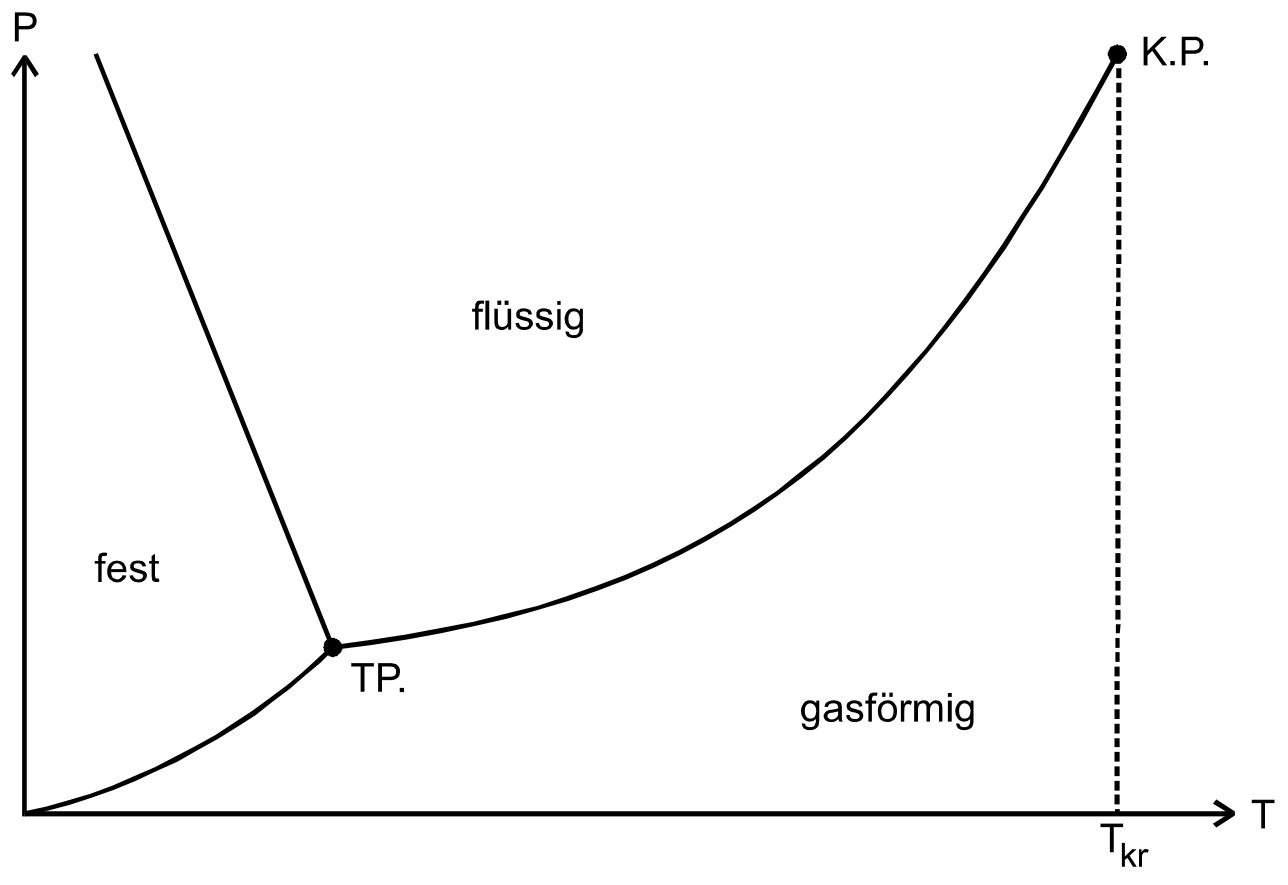
\includegraphics[width=\textwidth]{Bilder/Phasendiagramm.png}%citation hinzufügen
    \label{fig:phasendiagramm}
\end{figure}
\noindent Das Diagramm ist desweiteren in drei Bereiche aufgeteilt, die jeweils den festen, den flüssigen und den gasförmigen Zustand wiederspiegeln.
Der hier relevante Übergang, den zwischen dem flüssigen und gasförmigen Zustand wird als Dampfdruckkurve bezeichnet.
Sie verläuft zwischen den Punkten TP und KP, wobei KP der sogenannte kritische Punkt ist. Wenn nun ausschließlich die 
Dampfdruckkurve betrachtet wird, dann reduziert sich der Freiheitsgrad des Systems auf einen, da nun die Temperatur und der
Druck einen direkten Zusammenhang über die Verdampfungswärme $L$ haben. Diese ist für jeden Stoff charakteristisch, aber auch 
von der Temperatur abhängig und somit keine Konstante. Es gibt allerdings einen Bereich, in dem $L$ annähernd konstant ist und
sie geht gegen 0, wenn sich der Stoff dem kritischen Punkt KP nähert.\\

\noindent Wenn eine Flüssigkeit in einen abgeschlossenen Behälter gebracht wird, dann verdampft ein Teil der Flüssigkeit, da einige Teilchen
nach der Maxwellverteilung für Geschwindigkeiten schnell genug sind, um sich von den Zwischenmolekularen Bindungen zu lösen. 
Entsprechend kondensieren Teilchen wieder durch Zwischenmolekulare Interaktionen. Wenn das System lang genug laufen gelassen
wird stellt sich ein Geeichgewicht ein, der Sättigungsdampf. Der von diesem Dampf verursachte Druck heißt Sättigungdruck.
Dabei wird dieser nicht über die allgemeine Gasgleichung
\begin{equation}
    pV=\symup{R}T
    \label{eqn:gas}
\end{equation}
beschrieben, wobei R die allgemeine Gaskonstante ist.\\

\noindent Qualitativ kann so ein Prozess aus kondensieren und verdampfen als Kreisprozess dargestellt werden, wie
in Abbildung \ref{kreisprozess} aufgezeichnet ist.
\begin{figure}[H]
    \centering
    \caption{Kreisprozess zwischen Kondensation und Verdampfung}%citation hinzufügen
    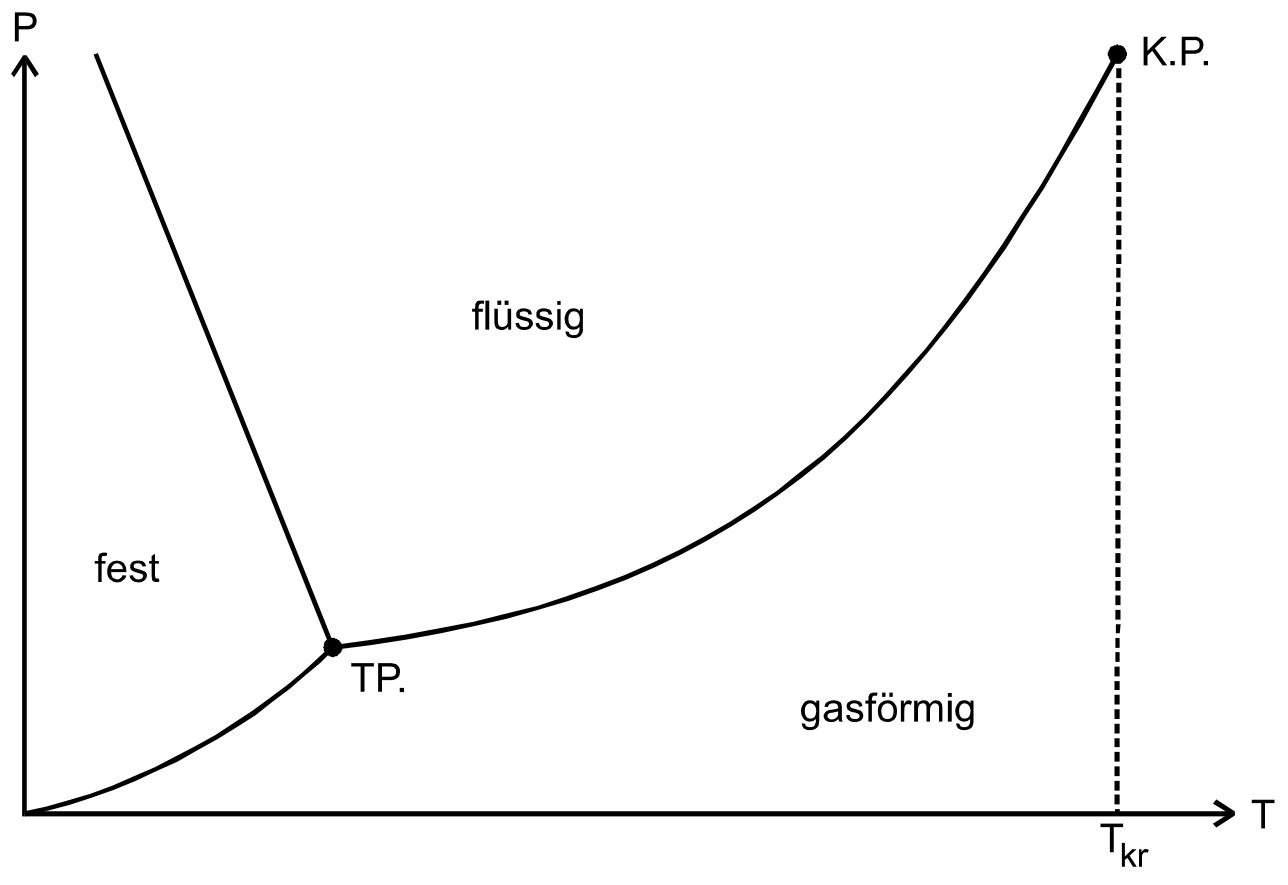
\includegraphics{Bilder/Phasendiagramm}
    \label{kreisprozess}
\end{figure}
\noindent Hier liegt in Punkt A nur eine Flüssigkeit vor, die durch Zufuhr von Verdampfungswärme $L$ auf B um $\symup{d}T$ erhitzt wird 
und dabei auf $V_F$ expandiert. In diesem Zustand verdampft die Flüssigkeit nun und befindet sich dann in Punkt C des Diagramms 
und ist dabei auf ein Volumen $V_D$ expandiert. Wenn das Gas von C auf D abgekühlt wird, kondensiert es in seinen Ursprungszustand 
zurück und gibt die Wärmemenge $L$ wieder ab. Aus diesem Prozess lässt sich dann mithilfe des zweiten Hauptsatzes der Thermodynamik
auf Kreisprozesse angewendet
\begin{equation*}
    \sum_i \frac{Q_i}{T_i}=0
\end{equation*}
die Clausius-Clapexronische Diffentialgleichung
\begin{equation}
    (V_D-V_F)\symup{d}p=\frac{L}{T}\symup{d}T
    \label{eqn:clausius}
\end{equation}
herleiten.\\

\noindent Da sowohl die beiden Volumina $V_i$ und die Verdampfungswärme $L$ Funktionen von der Zeit sein können, werden zum 
Lösen der Gleichung die Annahmen getroffen, dass
\begin{itemize}
    \item $V_F$ gegenüber $V_D$ vernachlässigbar ist.
    \item $V_D$ sich mithilfe der idealen Gasgleichung \ref{eqn:gas} bestimmen lässt. 
    \item $L$ ist konstant gegenüber Veränderungen im Druck und der Temperatur.
\end{itemize}

\noindent Beim Lösen der Gleichung mithilfe von Trennung der Variablen lässt sich dann feststellen, dass sich
\begin{equation*}
    \symup{ln}(p)=-\frac{L}{\symup{R}T}+C
\end{equation*}
ergibt, oder auch
\begin{equation}
    p=p_0 \symup{exp} \left(-\frac{L}{\symup{R}T}\right)
    \label{eqn:druck}
\end{equation}
mit eingesetzter Anfangsbedingung.

\cite{V203}

